% Autor: Leonhard Segger, Alexander Neuwirth
% Datum: 2017-10-30
\documentclass[
	% Papierformat
	a4paper,
	% Schriftgröße (beliebige Größen mit „fontsize=Xpt“)
	12pt,
	% Schreibt die Papiergröße korrekt ins Ausgabedokument
	pagesize,
	% Sprache für z.B. Babel
	ngerman
]{scrartcl}

% Achtung: Die Reihenfolge der Pakete kann (leider) wichtig sein!
% Insbesondere sollten (so wie hier) babel, fontenc und inputenc (in dieser
% Reihenfolge) als Erstes und hyperref und cleveref (Reihenfolge auch hier
% beachten) als Letztes geladen werden!

% Silbentrennung etc.; Sprache wird durch Option bei \documentclass festgelegt
\usepackage{babel}
% Verwendung der Zeichentabelle T1 (Sonderzeichen etc.)
\usepackage[T1]{fontenc}
% Legt die Zeichenkodierung der Eingabedatei fest, z.B. UTF-8
\usepackage[utf8]{inputenc}
% Schriftart
\usepackage{lmodern}
% Zusätzliche Sonderzeichen
\usepackage{textcomp}

% Mathepaket (intlimits: Grenzen über/unter Integralzeichen)
\usepackage[intlimits]{amsmath}
% Ermöglicht die Nutzung von \SI{Zahl}{Einheit} u.a.
\usepackage{siunitx}
% Zum flexiblen Einbinden von Grafiken (\includegraphics)
\usepackage{graphicx}
% Abbildungen im Fließtext
\usepackage{wrapfig}
% Abbildungen nebeneinander (subfigure, subtable)
\usepackage{subcaption}
% Funktionen für Anführungszeichen
\usepackage{csquotes}
\MakeOuterQuote{"}
% Zitieren, Bibliographie
\usepackage{biblatex}


% Zur Darstellung von Webadressen
\usepackage{url}
%chemische Formeln
\usepackage[version=4]{mhchem}
% siunitx: Deutsche Ausgabe, Messfehler getrennt mit ± ausgeben
\usepackage{floatrow}
\floatsetup[table]{capposition=top}
\usepackage{float}
% Verlinkt Textstellen im PDF-Dokument
\usepackage[unicode]{hyperref}
% "Schlaue" Referenzen (nach hyperref laden!)
\usepackage{cleveref}
\sisetup{
	locale=DE,
	separate-uncertainty
}
\bibliography{14Mo_O2_11-06-2018_References}

\begin{document}
	
	\begin{titlepage}
		\centering
		{\scshape\LARGE Versuchsbericht zu \par}
		\vspace{1cm}
		{\scshape\huge O2 - Mikrowellen \par}
		\vspace{2.5cm}
		{\LARGE Gruppe 14Mo \par}
		\vspace{0.5cm}
		
		{\large Alexander Neuwirth (E-Mail: a\_neuw01@wwu.de) \par}
		{\large Leonhard Segger (E-Mail: l\_segg03@uni-muenster.de) \par}
		\vfill
		
		durchgeführt am 11.06.2018\par
		betreut von\par
		{\large Stephan Majert}
		
		\vfill
		
		{\large \today\par}
	\end{titlepage}
	\tableofcontents
	\newpage

	%TODO mehr TODO in Default	

	\section{Kurzfassung}
	%TODO Hypothese	und deren Ergebnis, wenn Hypothese ist, dass nur Theorie erfüllt, sagen: Erwartung: Theorie aus einführung (mit reflink) erfüllt
	%TODO Ergebnisse, auch Zahlen, mindestens wenn's halbwegs Sinn ergibt
	%TODO Was wurde gemacht
	%TODO manche leute wollen Passiv oder "man", manche nicht
	Mikrowellen sind elektromagnetische Wellen im Bereich von etwa \SI{1}{\giga \Hz} bis etwa \SI{300}{\giga \hertz}.
	Um verschiedene Eigenschaften von Mikrowellen im Allgemeinen und der vorliegenden Mikrowellenquelle im Speziellen zu untersuchen, werden mehrere Untersuchungen durchgeführt. %TODO Untersuchuungen => Experimente ( sonst doppelt)
	Es wird vermutet, dass es sich bei dem durch die vorliegende Mikrowellenquelle ausgesendeten Strahl um einen Gauß-Strahl handelt.
	Hierzu wird die Divergenz des Strahls bestimmt und der Vergleich mit der für einen Gauß-Strahl erwarteten Divergenz bestätigte diese Vermutung.
	Außerdem kann durch senkrechtes Bestrahlen einer Metallplatte aus den Abständen der Minima der Intensität bei Erzeugung einer stehenden Welle die Wellenlänge der von der vorliegenden Quelle ausgesendeten Strahlung bestimmt werden. %TODO Komma
	Diese Wellenlänge liegt erwartungsgemäß im Mikrowellenbereich.
	Es wird vermutet, dass sich Mikrowellen bei der Brechung an dem Übergang von Luft zu PVC und PVC zu Luft gemäß des Snelliusschen Brechungsgesetz verhalten.
	Dies kann gezeigt werden, indem der gemessene Brechungsindex mit dem gemäß eines Literaturwert erwarteten verglichen wird.
	Auch das Phänomen der frustrierten Totalreflexion wird untersucht und der zu erwartende exponentielle Abfall beobachtet.
	Zuletzt wird die Bragg-Reflexion betrachtet und gezeigt, dass sich dieses Phänomen an einem Schaumstoffquader, der mit einem dreidimensionalen Gitter aus Metallkugeln gefüllt ist, beobachten lässt.
	
	%TODO Vgl. Bestrahlung beide Seiten Halbzylinder Hyp
	\section{Methoden}
	Es wird der Mikrowellensender auf einer Schiene und der Empfänger auf  einer sich dazu senkrecht befindenden befestigt.
	Dann wird durch Drehung des Senders um die Strahlungsachse die Polarisationsebene geändert, bis die vom Empfänger gemessene Intensität maximal ist.
	Die Intensität am Empfänger wird für unterschiedliche Abstände des Empfängers von der Strahlungsachse gemessen (Y-Achse).
	Diese Geometrie ist in \cref{fig_mikrowellenmitachsen} dargestellt.
	Dies wird für unterschiedliche Abstände des Senders zur orthogonalen Schiene des Empfängers (X-Achse) durchgeführt, um den virtuellen Quellfleck des Senders bestimmen zu können.
	
	Dann wird eine Metallplatte in den Strahlengang gebracht, sodass sie die Strahlung reflektieren und eine stehende Welle bilden kann.
	Während mit einem Empfänger nach den Knoten gesucht wird, wird der Abstand der Metallplatte zur Quelle optimiert, bis die Knoten möglichst gut ausgebildet sind, also die Intensität möglichst nah an Null liegt.
	Die Positionen mehrerer Knoten wird gemessen, um daraus die Wellenlänge bestimmen zu können. %TODO sollte man so Sinn angeben?
	
	Ein PVC-Halbzylinder wird anstelle der Platte in den Strahlengang gebracht.
	Dieser ist drehbar gelagert, sodass der Einfallswinkel variabel ist.
	Für mehrere Einfallwinkel wird mit einem Empfänger der Winkel der maximalen Transmission gesucht und gemessen.
	Dies wird zweimal durchgeführt.
	Dabei wird der Halbzylinder einmal so gedreht, dass die Welle erst durch die flache Seite des Halbzylinders einfällt und dann durch die runde ausfällt und einmal so, dass es andersherum stattfindet.
	
	Dann wird der Halbzylinder so gedreht, dass die Mikrowelle zuerst auf die runde Seite einfällt und im Inneren an der flachen Seite Totalreflexion zu beobachten ist. %TODO ist dass zu unpräzise? KP
	Ein zweiter Halbzylinder wird auf die Transmissionsseite des ersten gebracht, sodass die flachen Seiten einander zugewandt sind, und die Intensität der Strahlung hinter dem zweiten Halbzylinder in Abhängigkeit vom Abstand der beiden Zylinder gemessen.
	
	Zuletzt wird ein Schaumstoffquader, in dem sich ein dreidimensionales Gitter aus Metallkugeln befindet, in den Strahlengang gebracht und bei variablem Einfallswinkel die Intensität am gleich groß gewählten Reflexionswinkel gemessen.
	
	Die Intensität wird bei all diesen Messungen mit einem Empfänger gemessen, der eine Spannung ausgibt, die proportional zur Intensität ist.
	
	\begin{figure}[H] 
		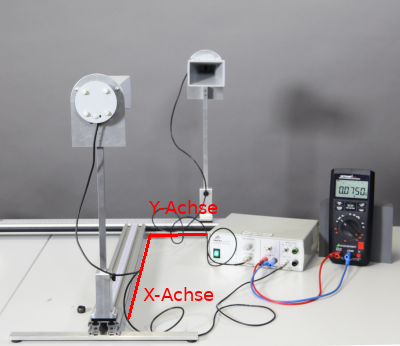
\includegraphics[width=0.7\textwidth]{MikrowellenMitAchsen}
		\centering
		\caption{Aufbau zur Bestimmung des Quellflecks mit Achsenbeschriftungen.\cite{Geometrie}}
		\label{fig_mikrowellenmitachsen}
		\centering
	\end{figure}
	
	\section{Ergebnisse und Diskussion}
	%TODO Unsicherheiten
	

	%TODO Einflüsse von veränderten Parametern auf Messung
	\subsection{Beobachtungen und Datenanalyse}
	\subsubsection{Unsicherheiten} %TODO GGF IN DATENANYLSY
	Die Unsicherheiten werden gemäß GUM ermittelt. 
	Außerdem wird für Unsicherheitsrechnungen die Python Bibliothek "uncertainties" verwendet.
	\begin{description}
		\item[Messleiste:] Die Unsicherheit der Messleiste wird auf \SI{0,2}{cm} abgeschätzt (dreieckige WDF).
		\item[Maßband/Geodreieck:] Die Unsicherheit von Maßband und Geodreieck wird mit \SI{0,05}{cm} bemessen (dreieckige WDF).
		\item[Winkelmessung:]  Die Winkel werden mit dem Auge anhand einer Skala abgelesen, wobei die Unsicherheit \SI{0,4}{\degree} beträgt. Beim Verstellen des Winkelmessarmes hat dieser jedoch viel Spielraum, in dem sich der Winkelzeiger nicht verändert hat. Deshalb wird für diese Messung die doppelte Unsicherheit gewählt.
		\item[Multimeter:] Das Multimeter zeigt die Spannung mit 2 Nachkommastellen an. Da bei den Messungen die Anzeige der letzten Ziffer schwankt, wird die Unsicherheit mit \SI{0,03}{V} abgeschätzt (rechteckige WDF).
	\end{description}

	\subsubsection{Bestimmung des Quellflecks des Senders}
	Es wird in vier verschiedenen Abständen zum Sender in orthogonaler Richtung elfmal die Intensität gemessen.
	Die gemessenen Strahlenprofile sind in \crefrange{fig_74cm}{fig_114cm} dargestellt. 
	\begin{figure}[H]
		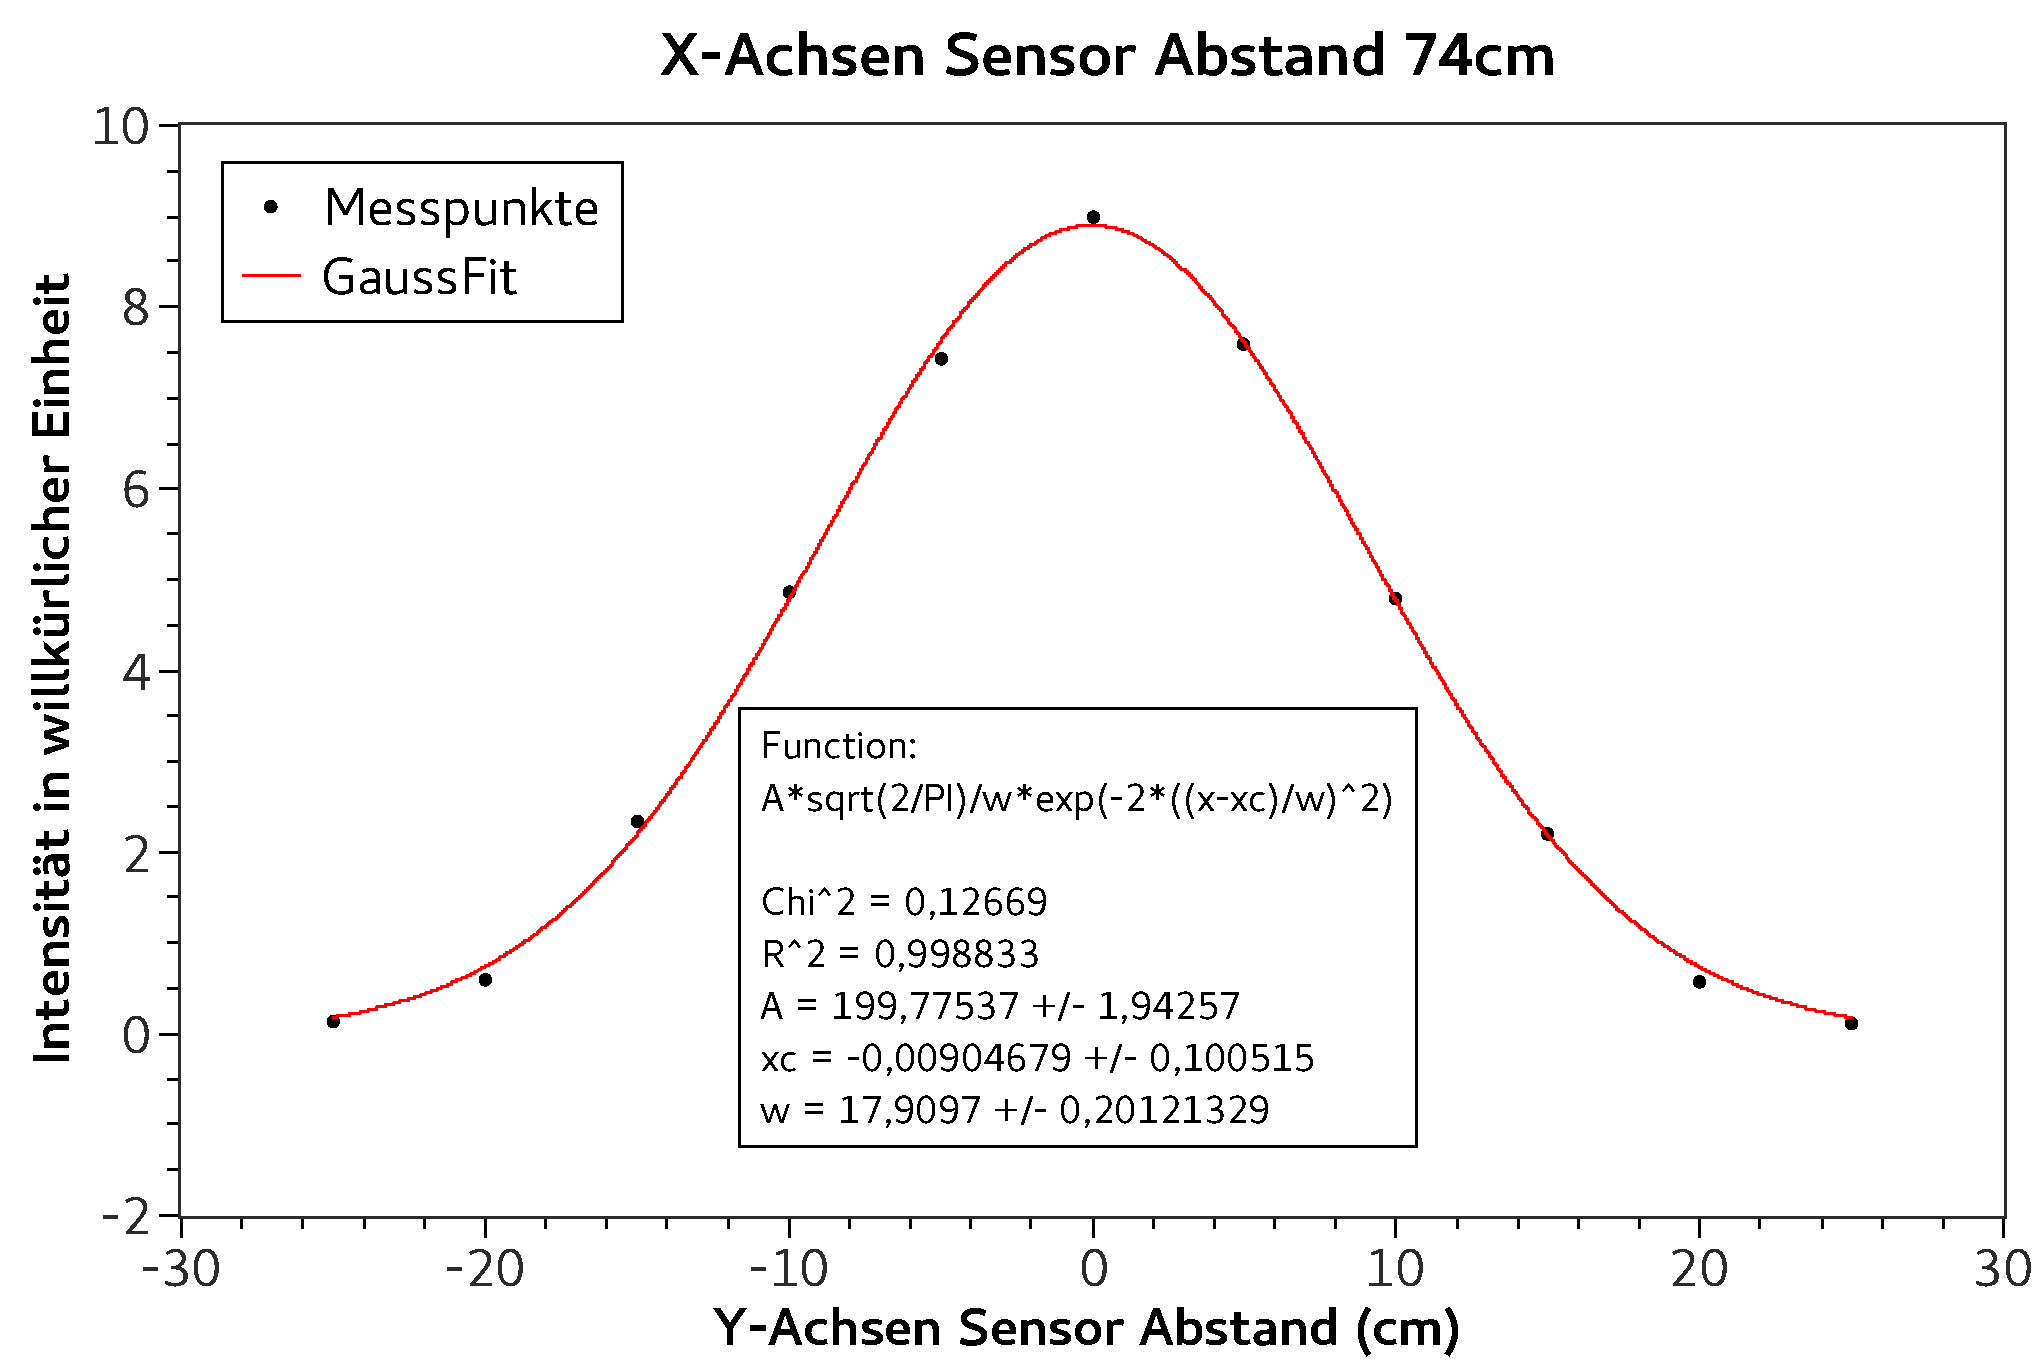
\includegraphics[width=0.7\textwidth]{fig_74cm_gauss}
		\centering
		\caption{Strahlenprofil im Abstand von \SI{74}{cm}. Die Unsicherheiten sind kleiner als die Symbolgröße.}
		\label{fig_74cm}
		\centering
	\end{figure}

	\begin{figure}[H]
		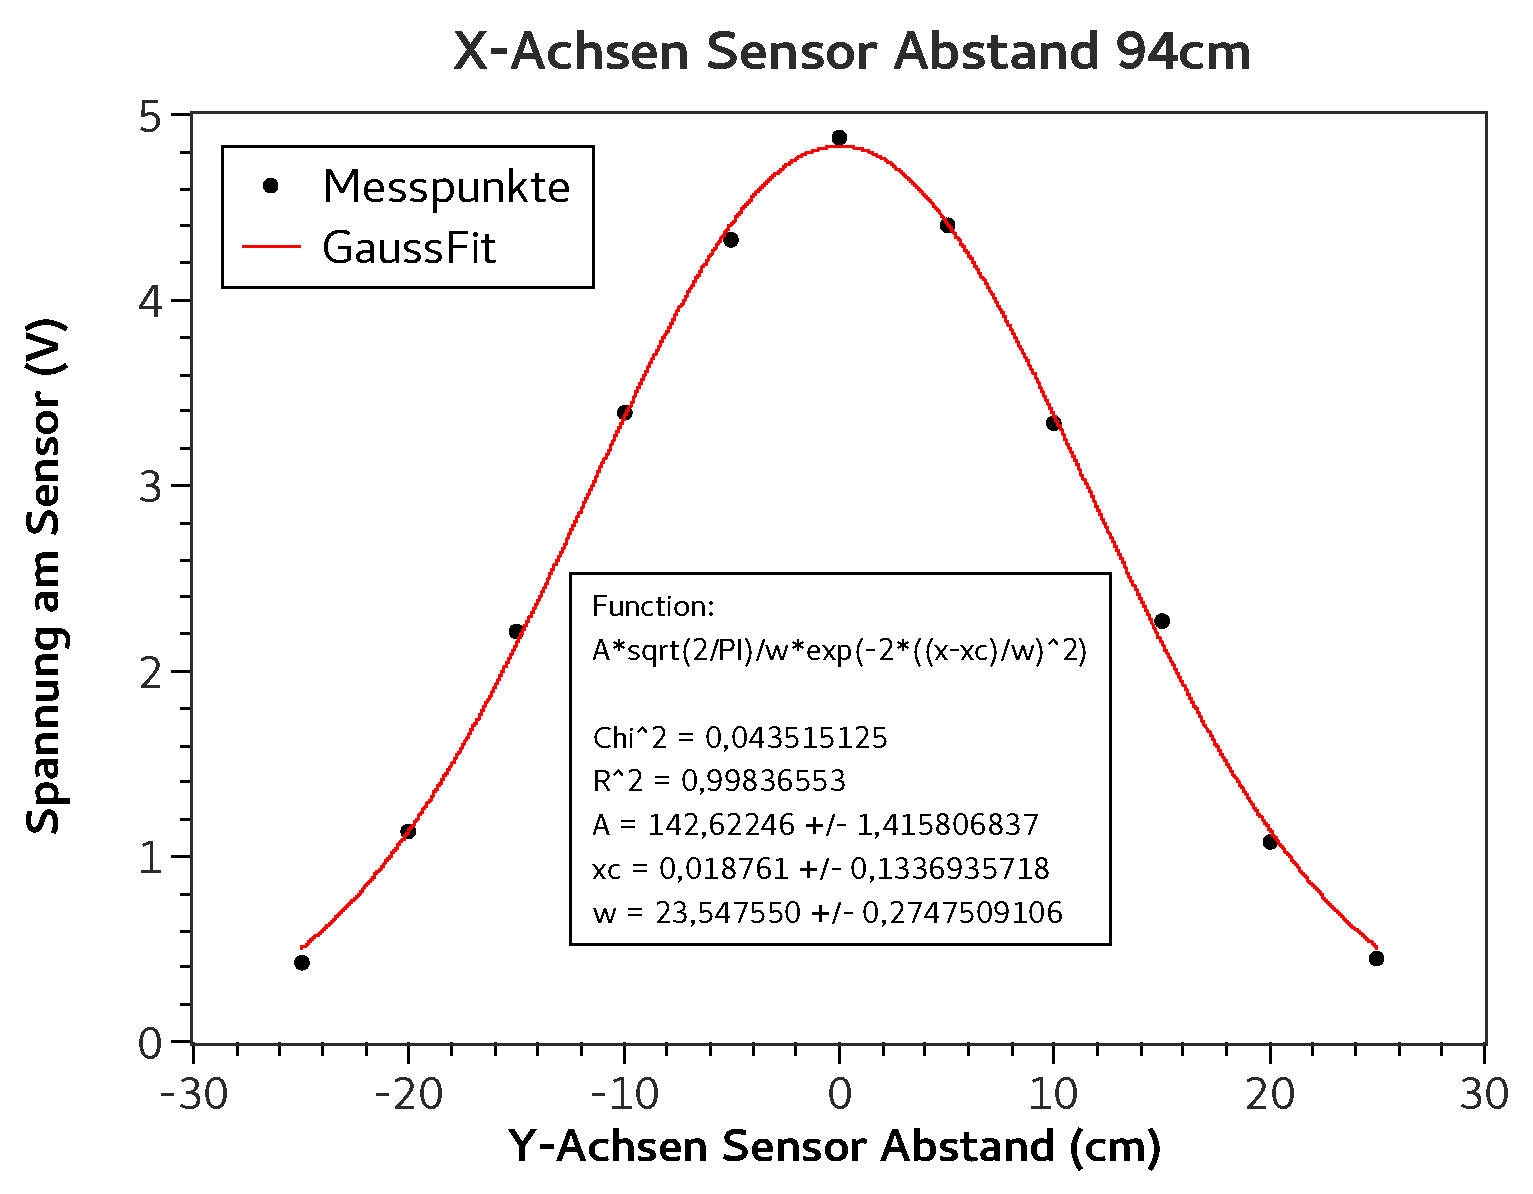
\includegraphics[width=0.7\textwidth]{fig_94cm_gauss}
		\centering
		\caption{Strahlenprofil im Abstand von \SI{94}{cm}. Die Unsicherheiten sind kleiner als die Symbolgröße.}
		\label{fig_94cm}
		\centering
	\end{figure}
	\begin{figure}[H]
		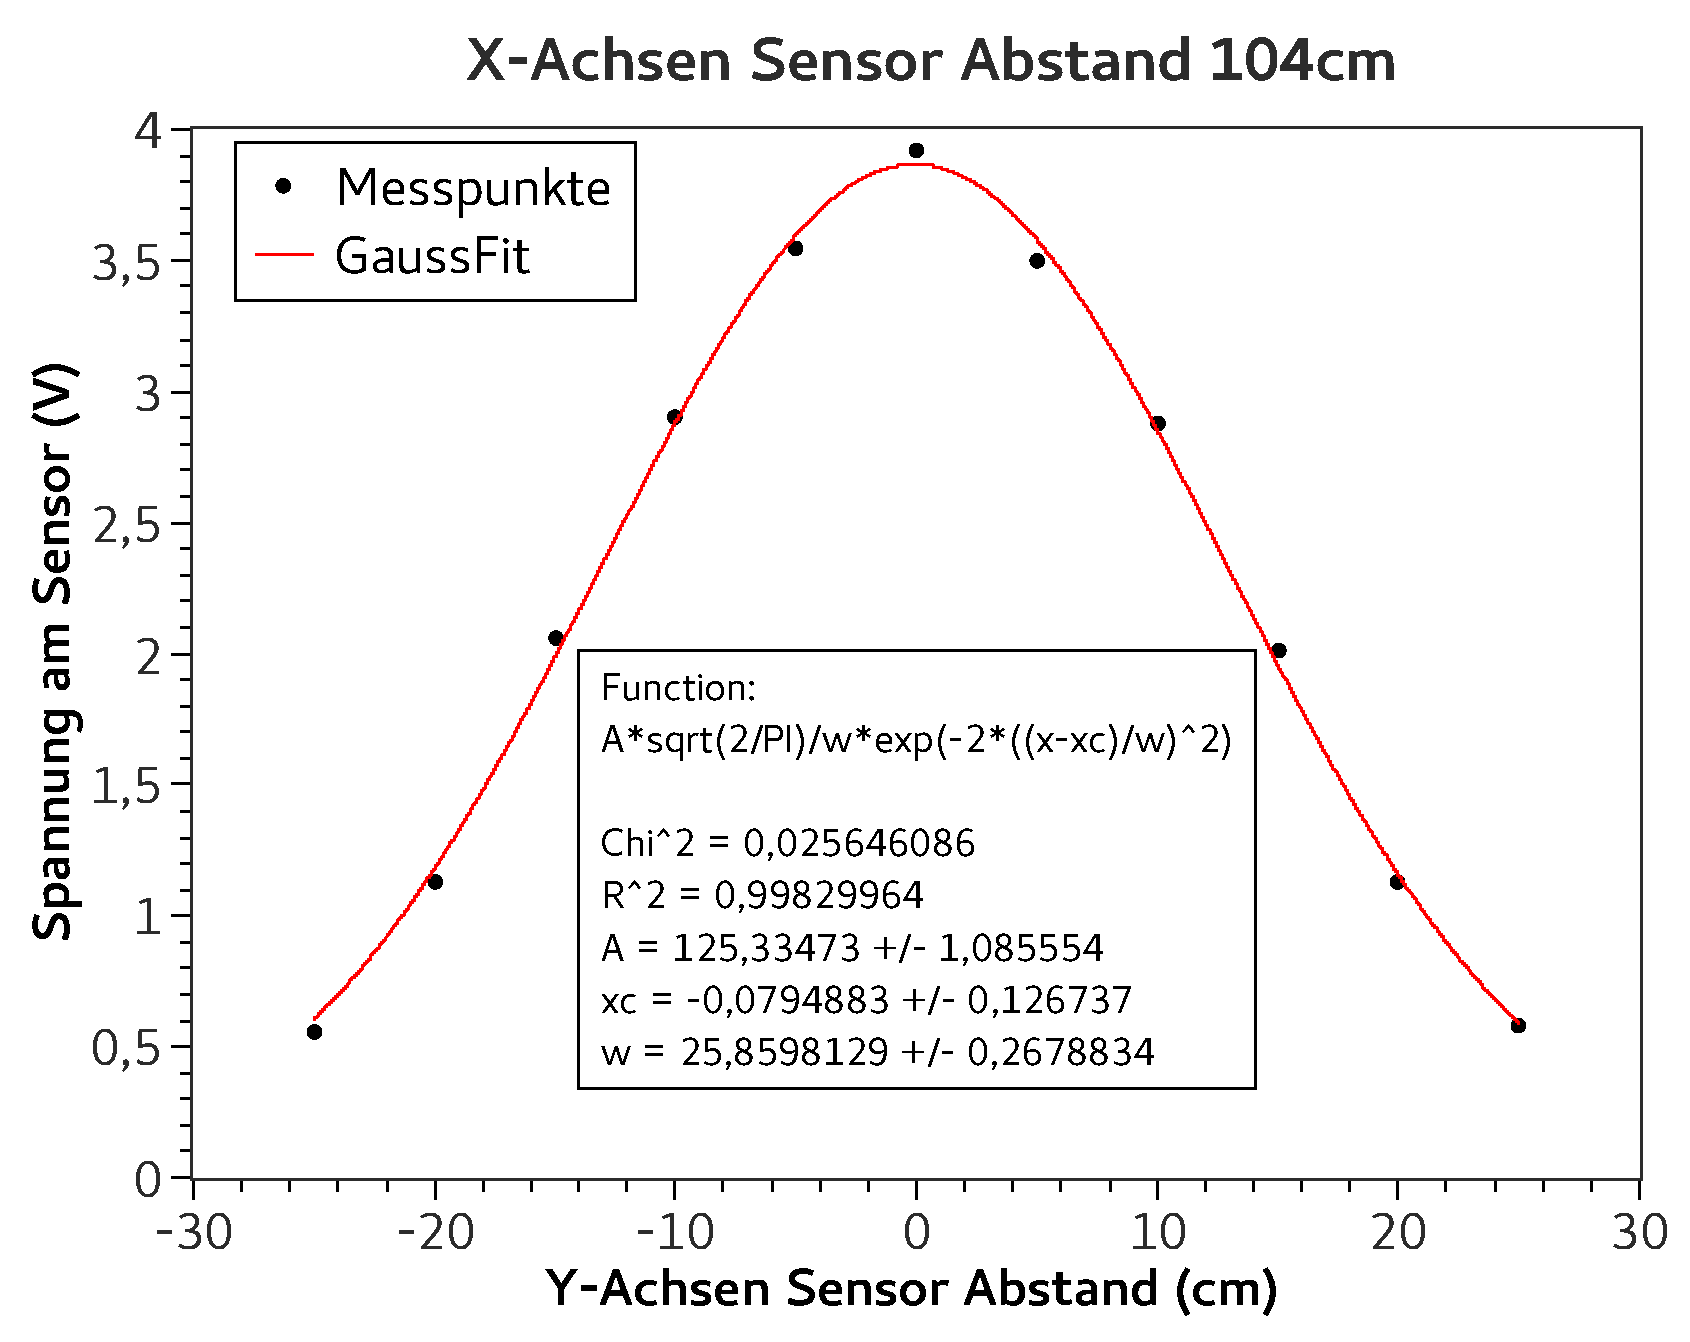
\includegraphics[width=0.7\textwidth]{fig_104cm_gauss}
		\centering
		\caption{Strahlenprofil im Abstand von \SI{104}{cm}. Die Unsicherheiten sind kleiner als die Symbolgröße.}
		\label{fig_104cm}
		\centering
	\end{figure}
	\begin{figure}[H]
		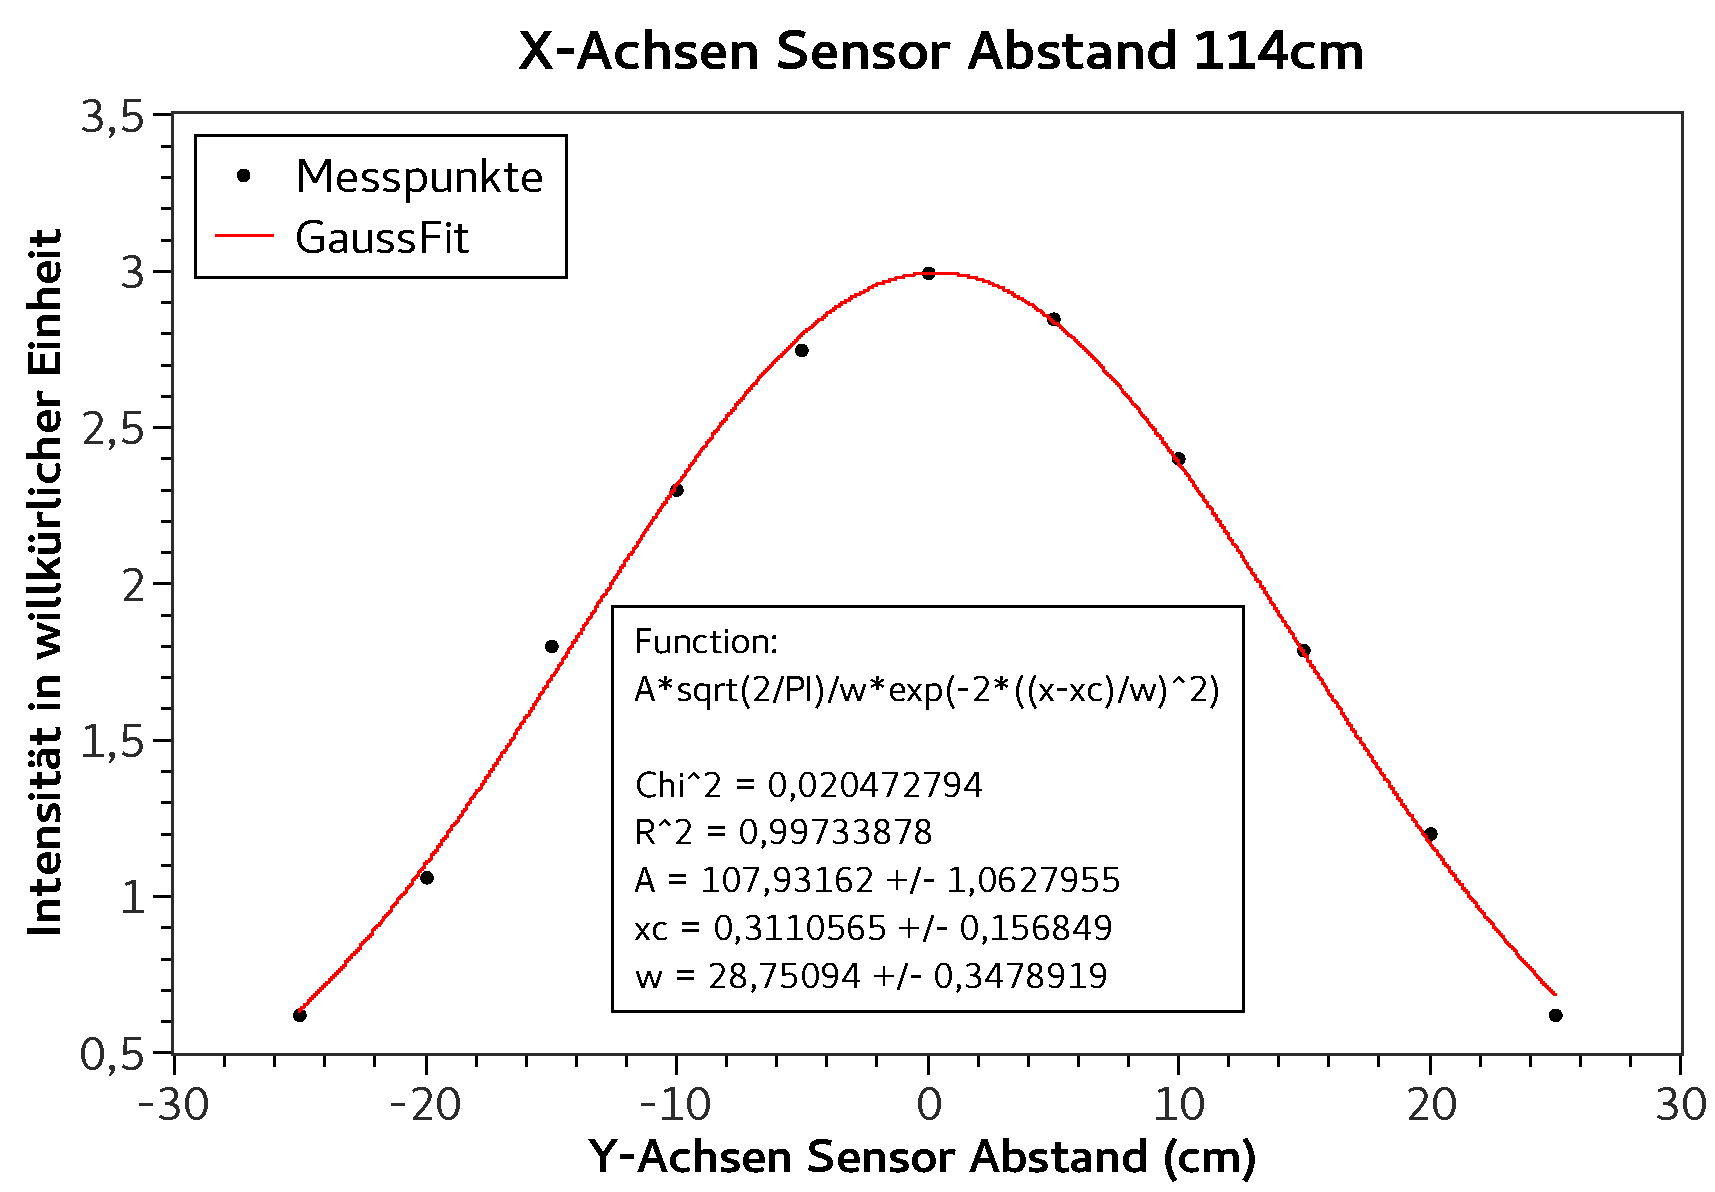
\includegraphics[width=0.7\textwidth]{fig_114cm_gauss}
		\centering
		\caption{Strahlenprofil im Abstand von \SI{114}{cm}. Die Unsicherheiten sind kleiner als die Symbolgröße.}
		\label{fig_114cm}
		\centering
	\end{figure}
	Um die Hypothese, dass der Sender einen Gauß-Strahl aussendet, zu überprüfen, wird ein Gaußkurven-Fit durchgeführt. 
	Die resultierenden $xc$ in den Graphen sind die Abweichung des Quellflecks entlang der Y-Achse (\cref{fig_mikrowellenmitachsen}). 
	Diese sind in \cref{tab_xc} aufgeführt:
	\begin{table}[H]
		\centering
		\begin{tabular}{ c | c }
			X-Achsen Abstand Sender/Empfänger in \SI{}{cm} & $xc$ in \SI{}{cm}  \\ \hline
			\SI{74}{}&\SI{-0,01+-0,10}{}\\
			\SI{94}{}&\SI{0,02+-0,13}{}\\
			\SI{104}{}&\SI{-0,08+-0,13}{}\\
			\SI{114}{}&\SI{0,31+-0,16}{}\\
		\end{tabular}
		\caption{Zur Strahlungsrichtung orthogonale Abweichung $xc$ des Quellpunkts zum Sender.}
		\label{tab_xc} 
	\end{table}

	Die Halbwertsbreiten der Strahlenprofile beträgt: 
	\begin{equation}
		h = \sigma \cdot 2 \cdot \sqrt{2\cdot\ln(2)} = \omega \cdot \sqrt{2\cdot\ln(2)}.
	\end{equation}
	In \cref{fig_divergenz} sind die Halbwertsbreiten des Strahls gegen den X-Achsen Abstand zwischen Sender und Empfänger aufgetragen.
	Die Steigung des linearen Fits ist die Strahlungsdivergenz $S = \SI{0,317+-0,007}{}$.
	Die Verschiebung des Quellflecks zum Sender parallel zur Strahlungsrichtung lässt sich aus der Bedingung, in welchem Abstand $x$ $ax+b=0$ erfüllt, also an dem die Breite des Strahls minimal wird, berechnen. %holymoly alter
	Es folgt $x=\SI{7,2+-2,4}{cm}$.
	Das heißt der Quellfleck befindet sich \SI{7,2+-2,4}{cm} vor dem Sender (also näher am Empfänger).

	\begin{figure}[H]
		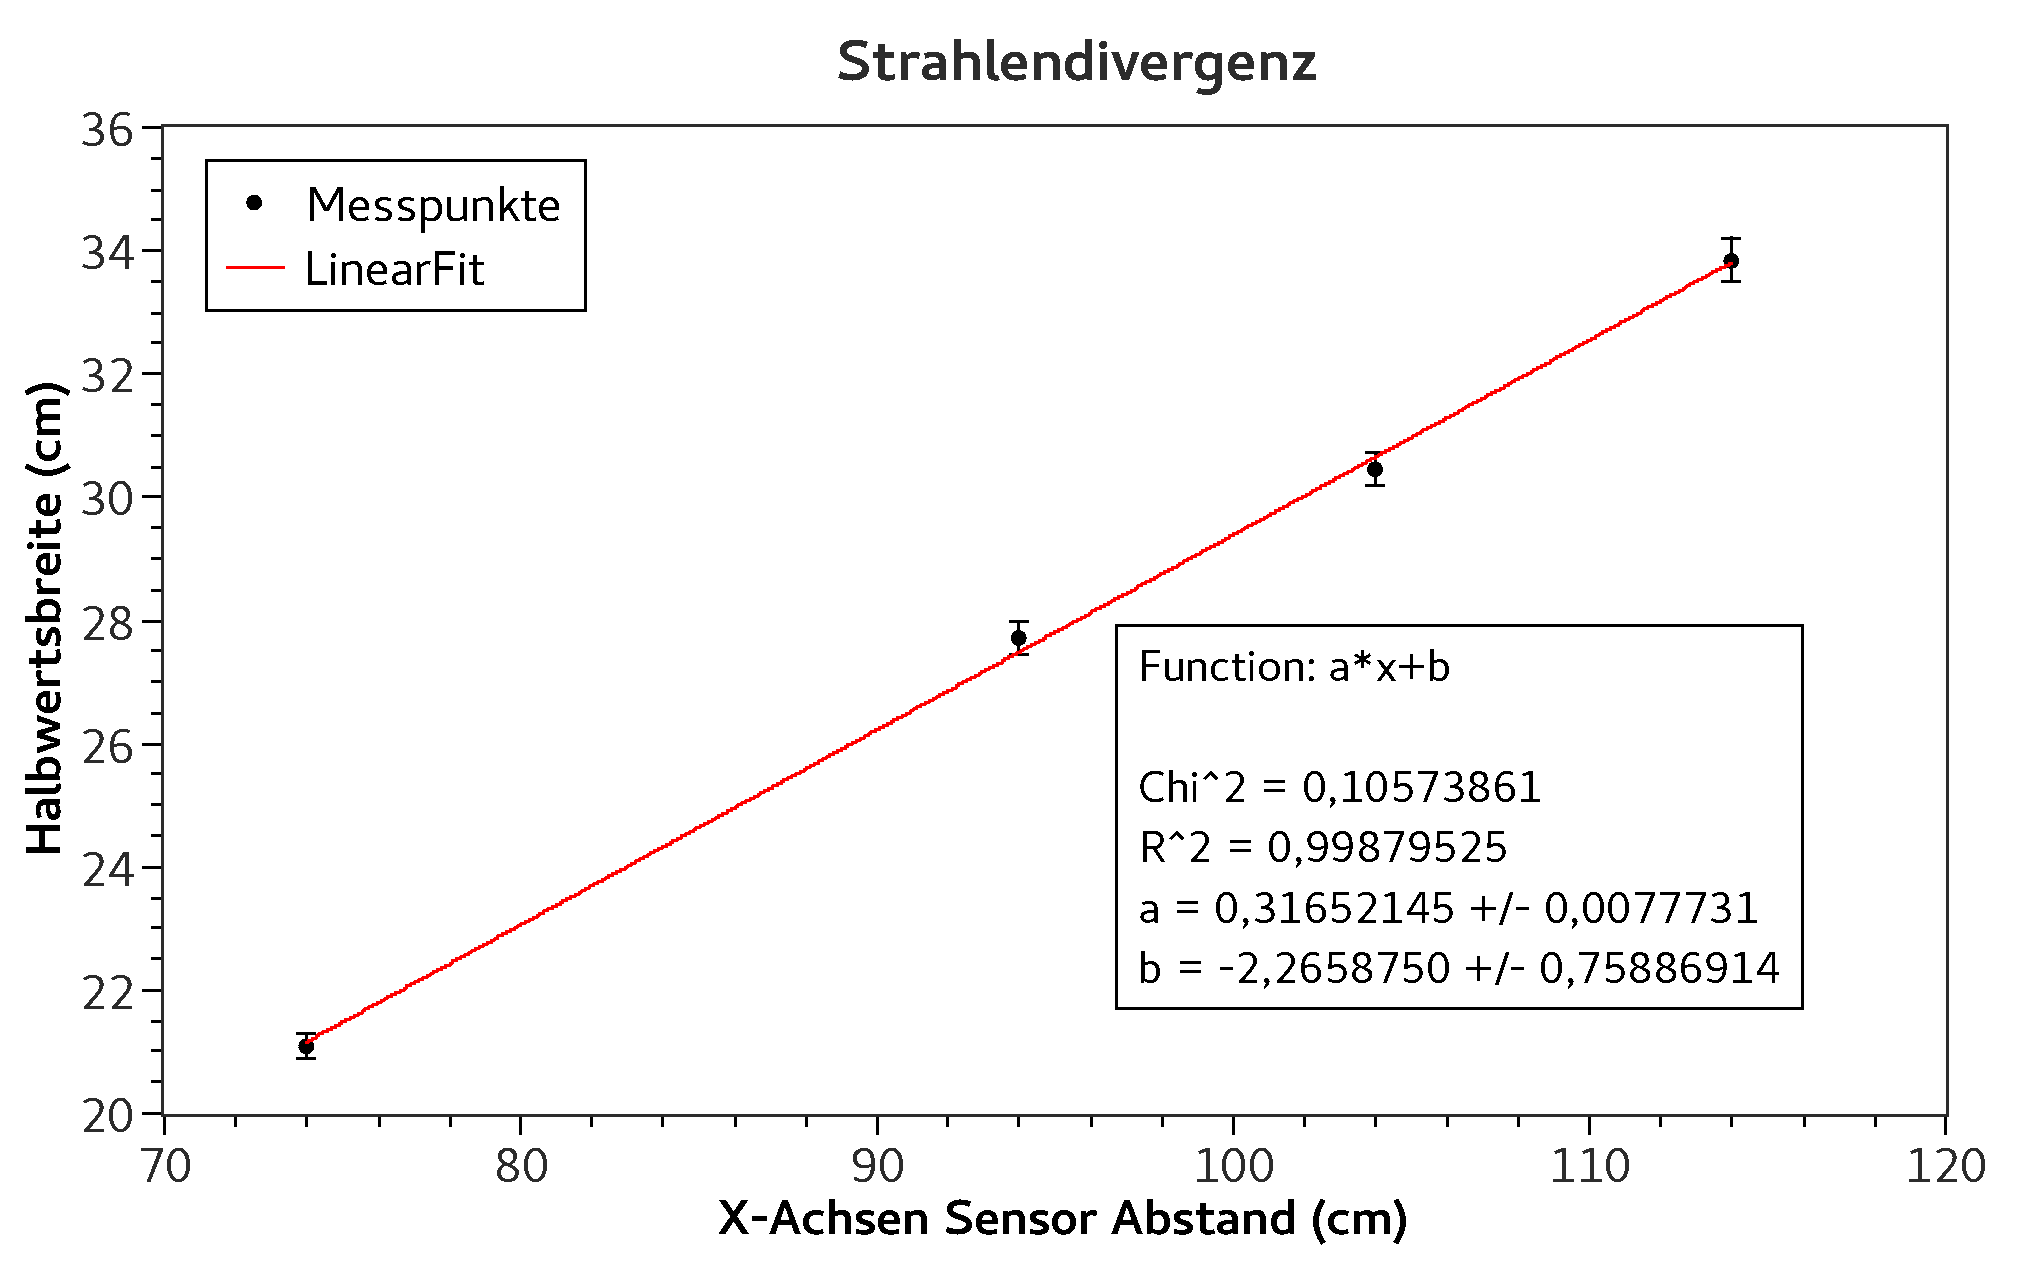
\includegraphics[width=1\textwidth]{fig_divergenz}
		\centering
		\caption{Die Halbwertsbreiten der Strahlenprofile sind gegen den Abstand des Sensors in X-Richtung aufgetragen.}
		\label{fig_divergenz}
		\centering
	\end{figure}
	
	\subsubsection{Bestimmung der Wellenlänge}
	Bei der bestmöglichen Auflösung der Knoten der stehenden Welle beträgt die Spannung an den Minima (Knoten) noch \SI{0,03}{V}.
	In \cref{fig_steh_welle} sind die Positionen der Minima aufgelistet.
	Die gemessenen Positionen der jeweiligen Strahlungsminima sind linear angeordnet. 
	Die gemittelte halbe Wellenlänge ergibt sich aus dem Abstand des ersten zum letzten Minimum geteilt durch die Anzahl der Minima. %Theoretisch wäre halt die einzelnen zu Mitteln möglicherweise präziser. - Nein, ich habe bsplw. auch nen Fit in den Graphen gemacht aber das ist halt ungenauer, weil er die Abstände zu den Punkten minimiert. Wenn man aber weiß, dass 10 Knoten drin sind, mitteln sich die einzelnen Abweichungen, wenn man nur die Grenzen anschaut gut weg. (Es konnte ja nicht ganz exakt der Knoten festgestellt werden
	So folgt: 
	\begin{equation}
		\lambda = 2 \cdot \frac{\SI{28,1 +- 0,2}{cm} + \SI{12,4+-0,2}{cm}}{10} = \SI{3,14 +- 0,05}{cm}.
	\end{equation}
	\begin{figure}[H]
		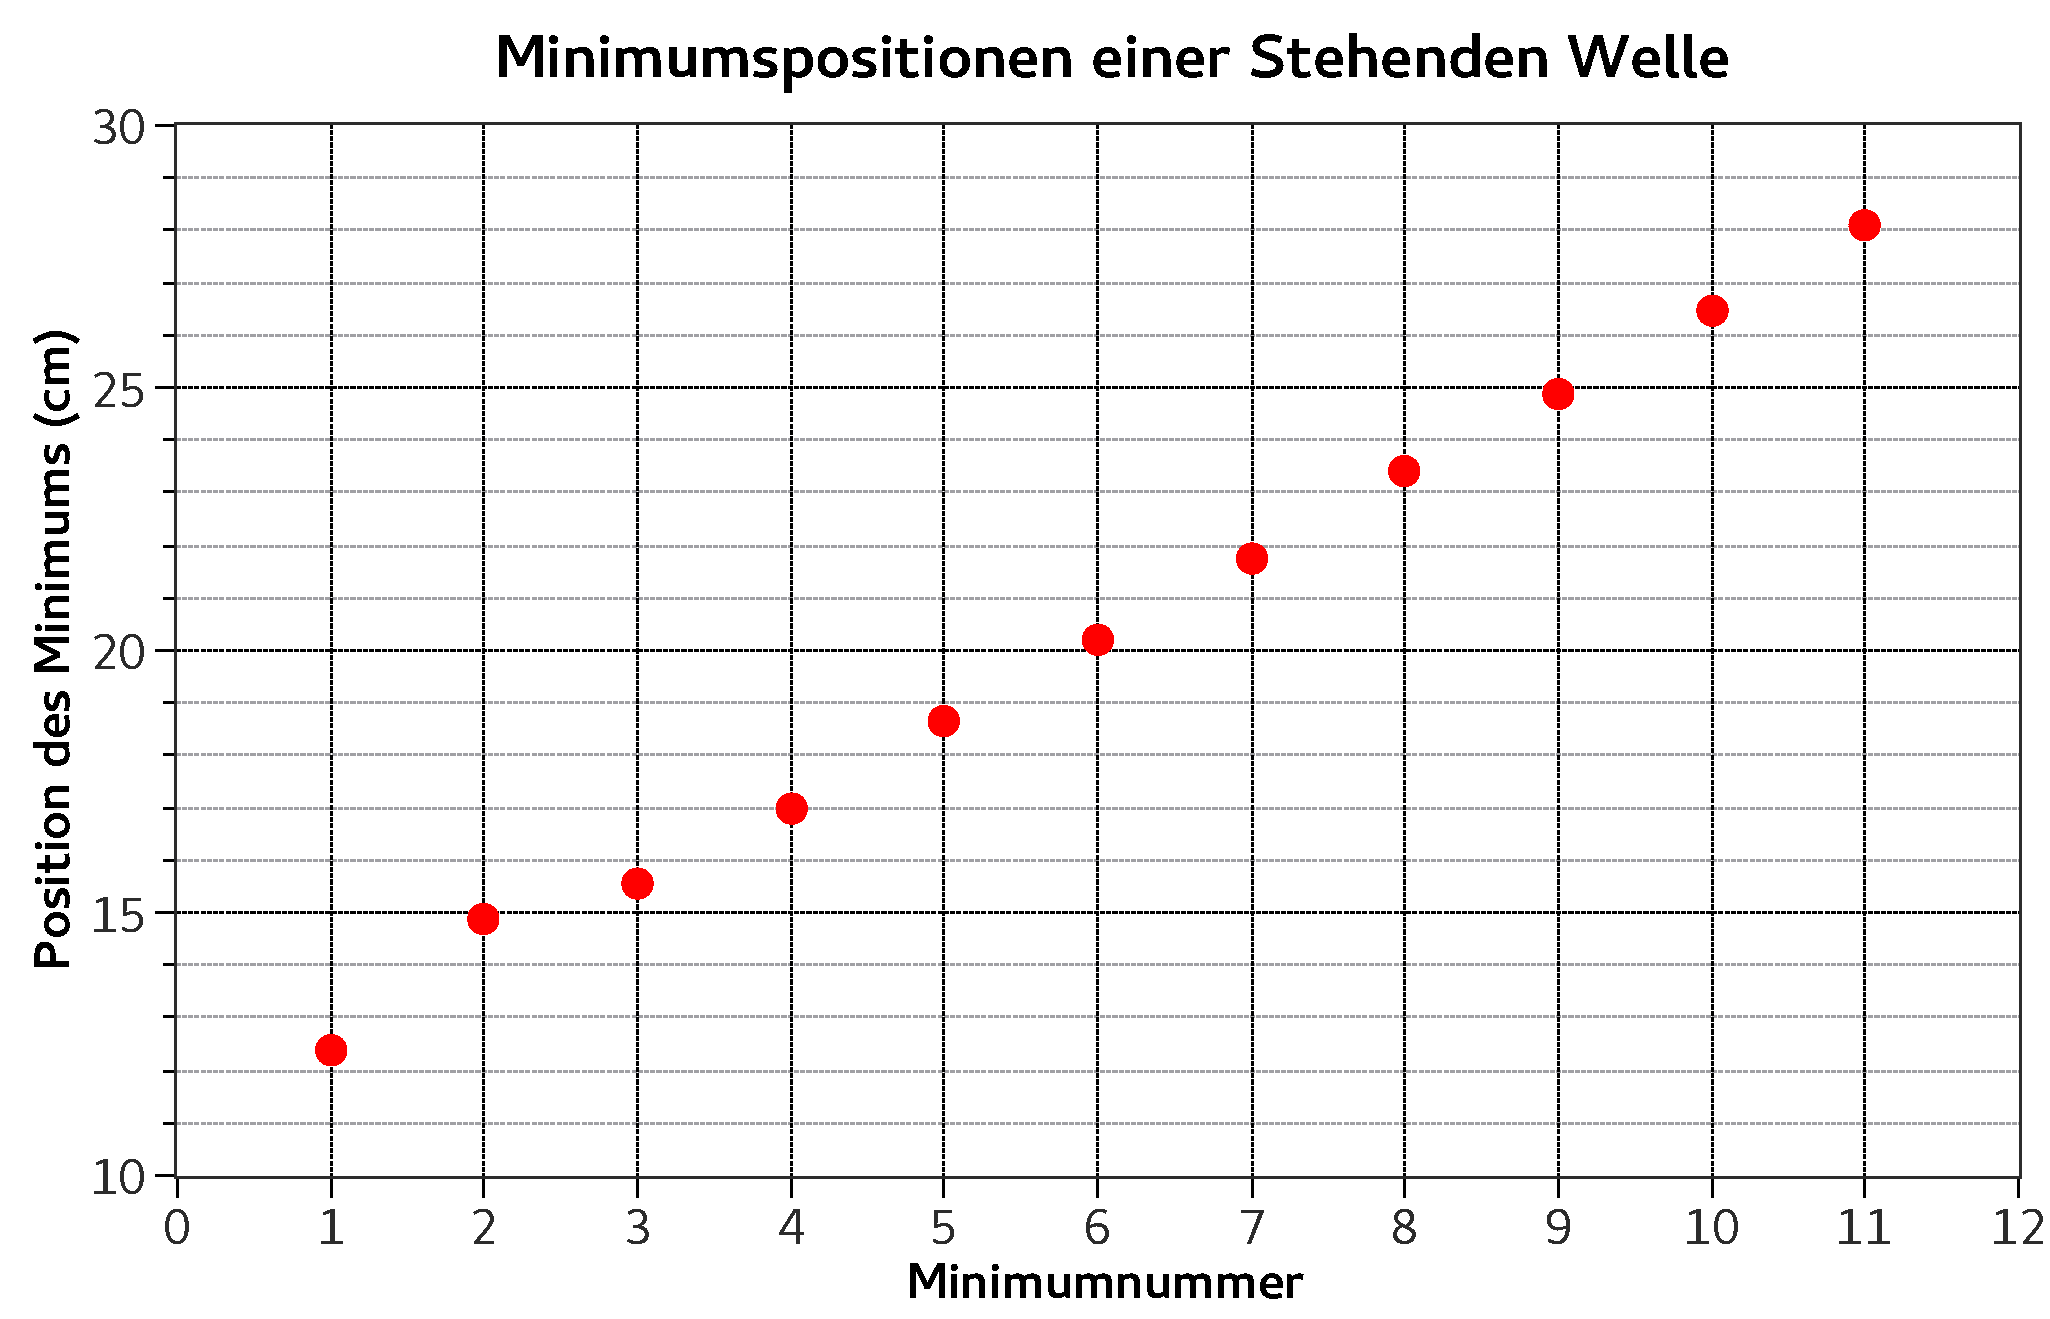
\includegraphics[width=0.7\textwidth]{fig_steh_welle}
		\centering
		\caption{Hier sind die gemessenen Positionen der Knoten der stehenden Welle dargestellt. Die Unsicherheiten sind kleiner als die Symbolgröße.}
		\label{fig_steh_welle}
		\centering
	\end{figure}
	\subsubsection{Bestimmung des Brechungsindex von PVC}
	Der Brechungsindex von PVC für Mikrowellen wird auf zwei Arten bestimmt. 
	Zuerst wird die runden Seite des Halbzylinders in verschiedenen Winkeln bestrahlt und der Winkel des Maximums der transmittierten Strahlung gemessen.
	Die Messergebnisse sind in \cref{fig_rund_zyl} aufgeführt.
	Das Snelliusschen Brechungsgesetz lautet:
	\begin{equation}
		n_i \cdot \sin(\vartheta_i) = n_t \cdot \sin(\vartheta_t)
		\label{eq_snellius}
	\end{equation}
	Somit kann der Brechungsindex $n_\text{PVC}$  mit 
	\begin{equation}
		n_\text{PVC} = \frac{\sin(\beta)}{\sin(\alpha)} n_\text{Luft}
	\end{equation}
	bestimmt werden.
	Da $n_\text{Luft}$ ungefähr 1 ist, ist die Steigung des linearen Fits in \cref{fig_rund_zyl} gleich $n_\text{PVC}=\SI{1,56 +- 0,05}{}$.

	\begin{figure}[H]
		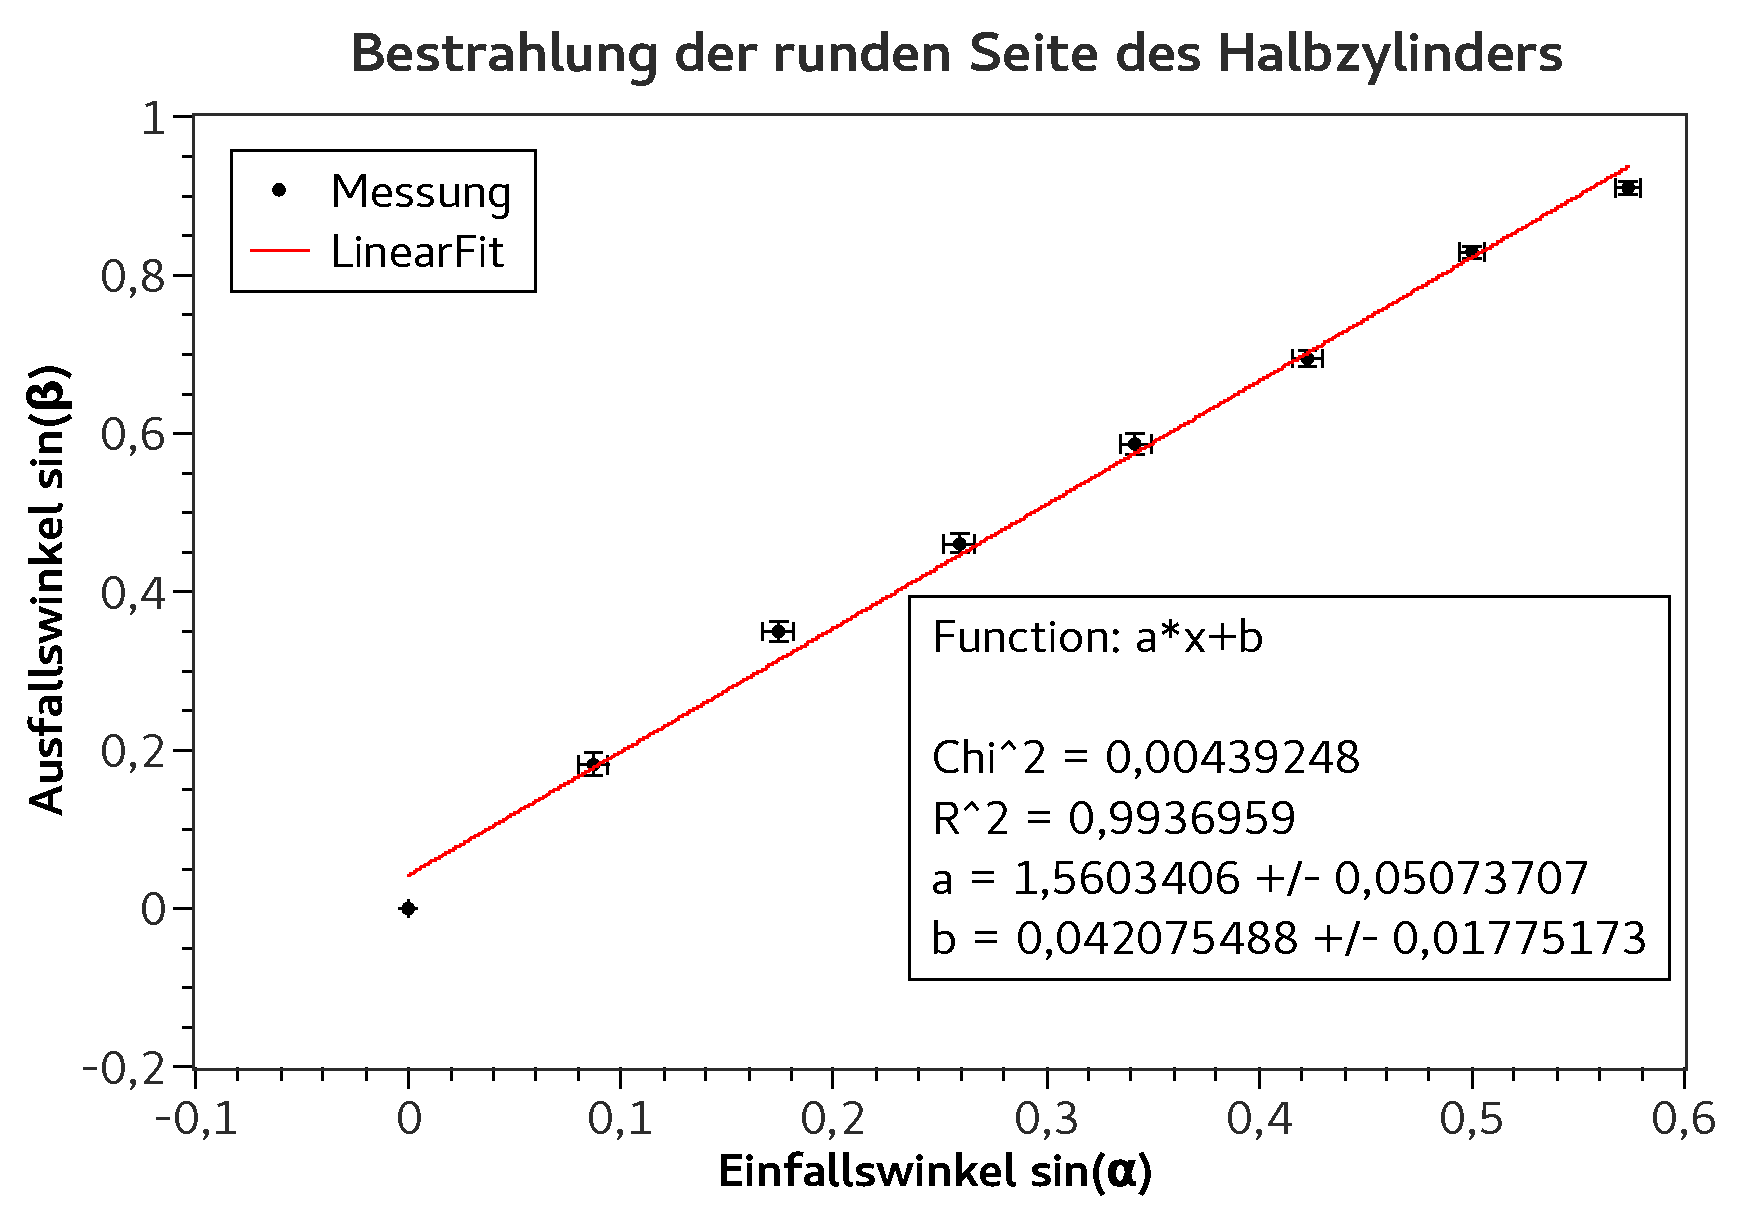
\includegraphics[width=0.7\textwidth]{fig_rund_zyl}
		\centering
		\caption{Der Sinus des Ausfallwinkels ist gegen den Sinus des Einfallwinkels beim Bestrahlen der runden Seite des Halbzylinders aus PVC aufgetragen.}
		\label{fig_rund_zyl}
		\centering
	\end{figure}

	Als zweite Messmethode wird die flache Seite des Halbzylinders bestrahlt.
	Die Rechnung erfolgt analog zur vorherigen, jedoch ist das Verhältnis der Sinusse der Winkel invertiert.
	Das heißt, die Steigung ist der Kehrwert des Brechungsindex von PVC.
	Aus der Steigung $a$ in \cref{fig_flach_zyl} von \SI{0,634+-0,020}{} folgt $n_\text{PVC} = \SI{1,57 +- 0,05}{}$.
	\begin{figure}[H]
		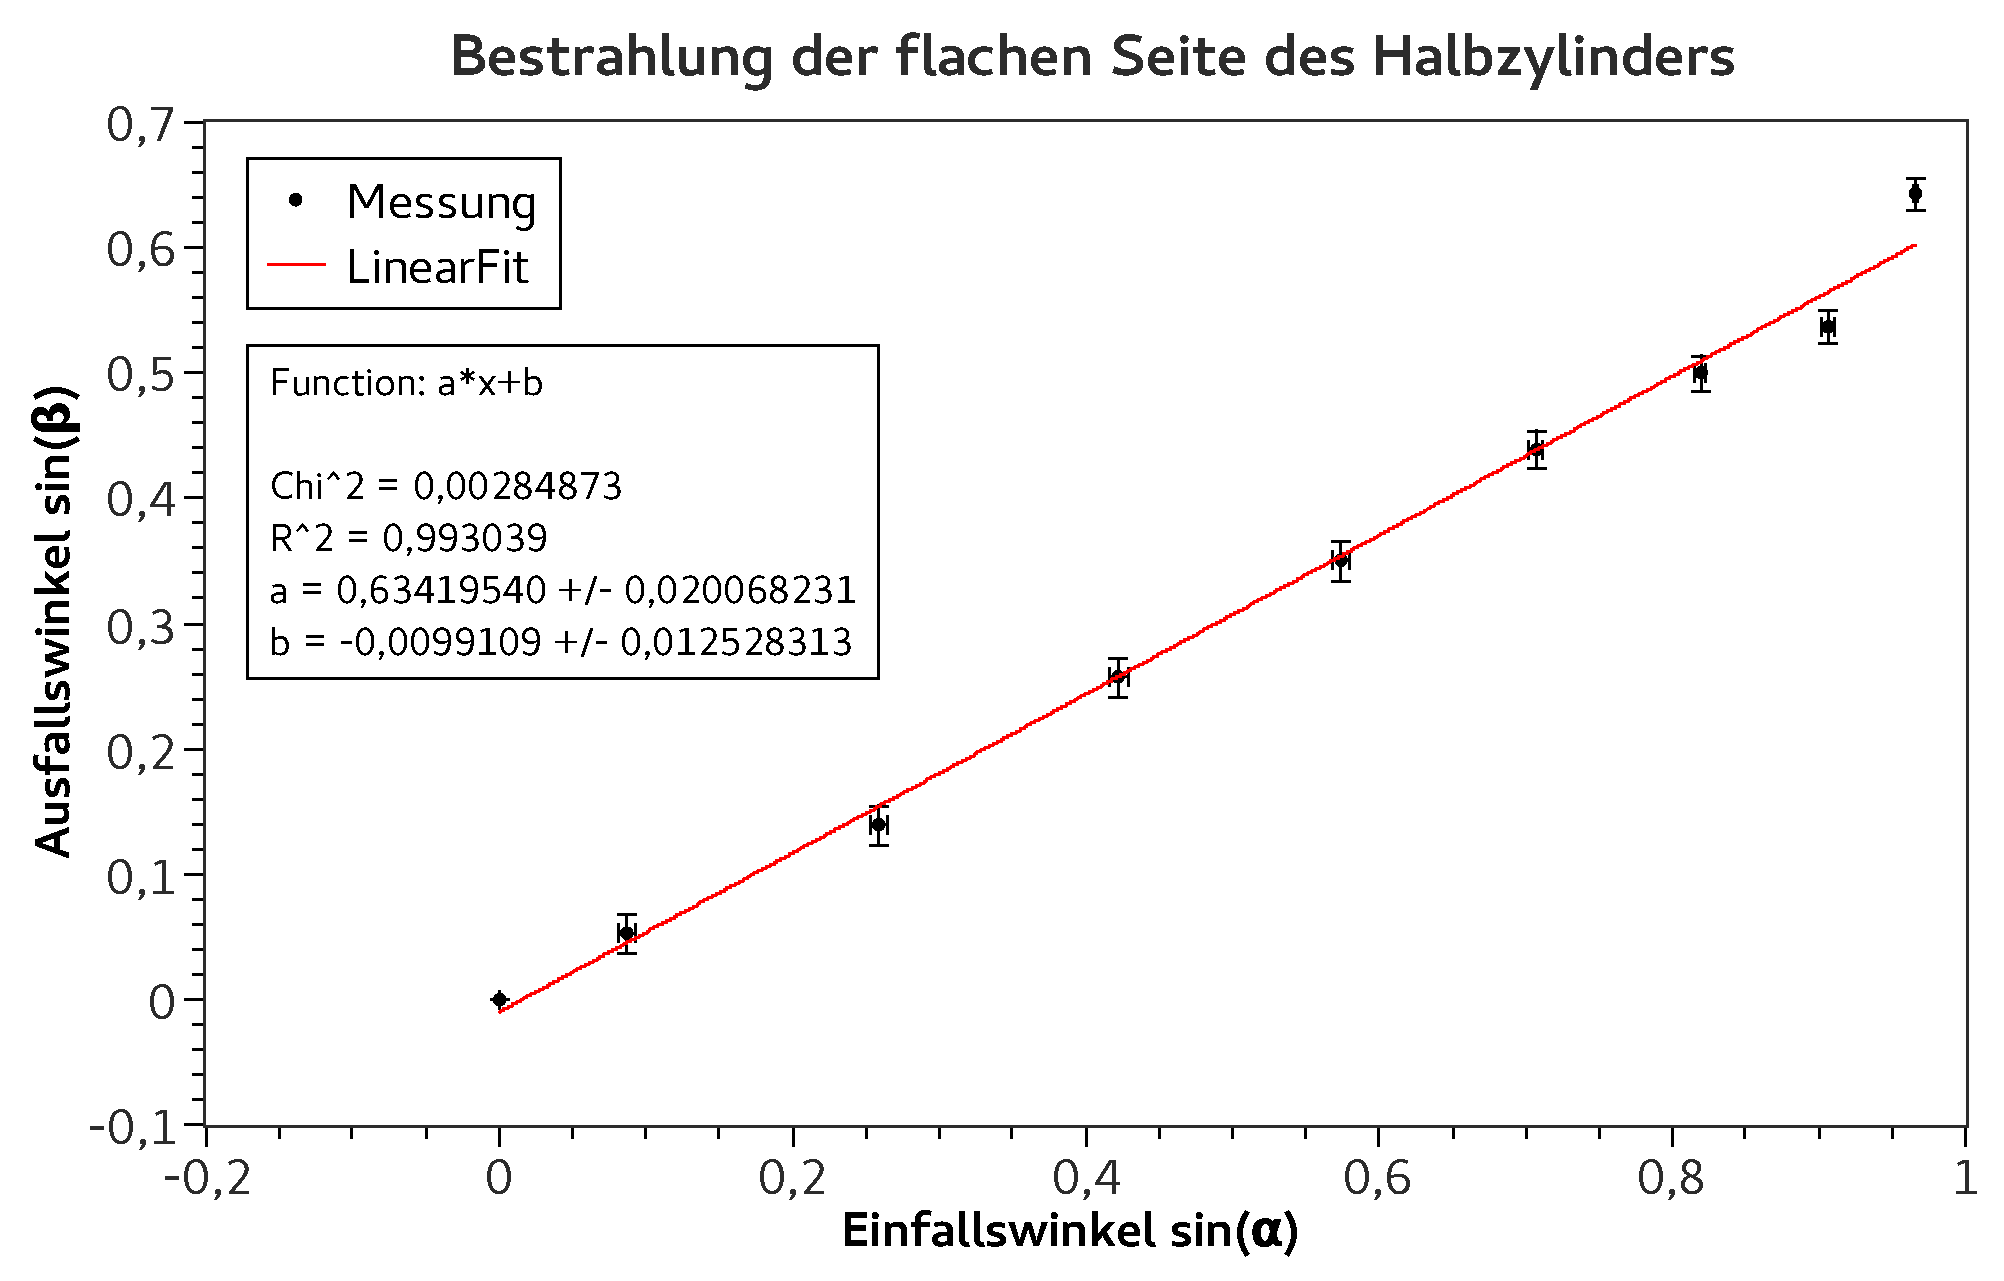
\includegraphics[width=0.7\textwidth]{fig_flach_zyl}
		\centering
		\caption{Der Sinus des Einfallwinkels $\alpha$ ist gegen den Sinus des Ausfallwinkels $\beta$, beim Bestrahlen der flachen Seite des Halbzylinders aus PVC, aufgetragen.}
		\label{fig_flach_zyl}
		\centering
	\end{figure}

	\subsubsection{Frustierte Totalreflexion}
	Es wird die Intensität der transmittierten Strahlung als Funktion der Lückenbreite gemessen und in \cref{fig_frust_total} abgebildet.
	\begin{figure}[H]
		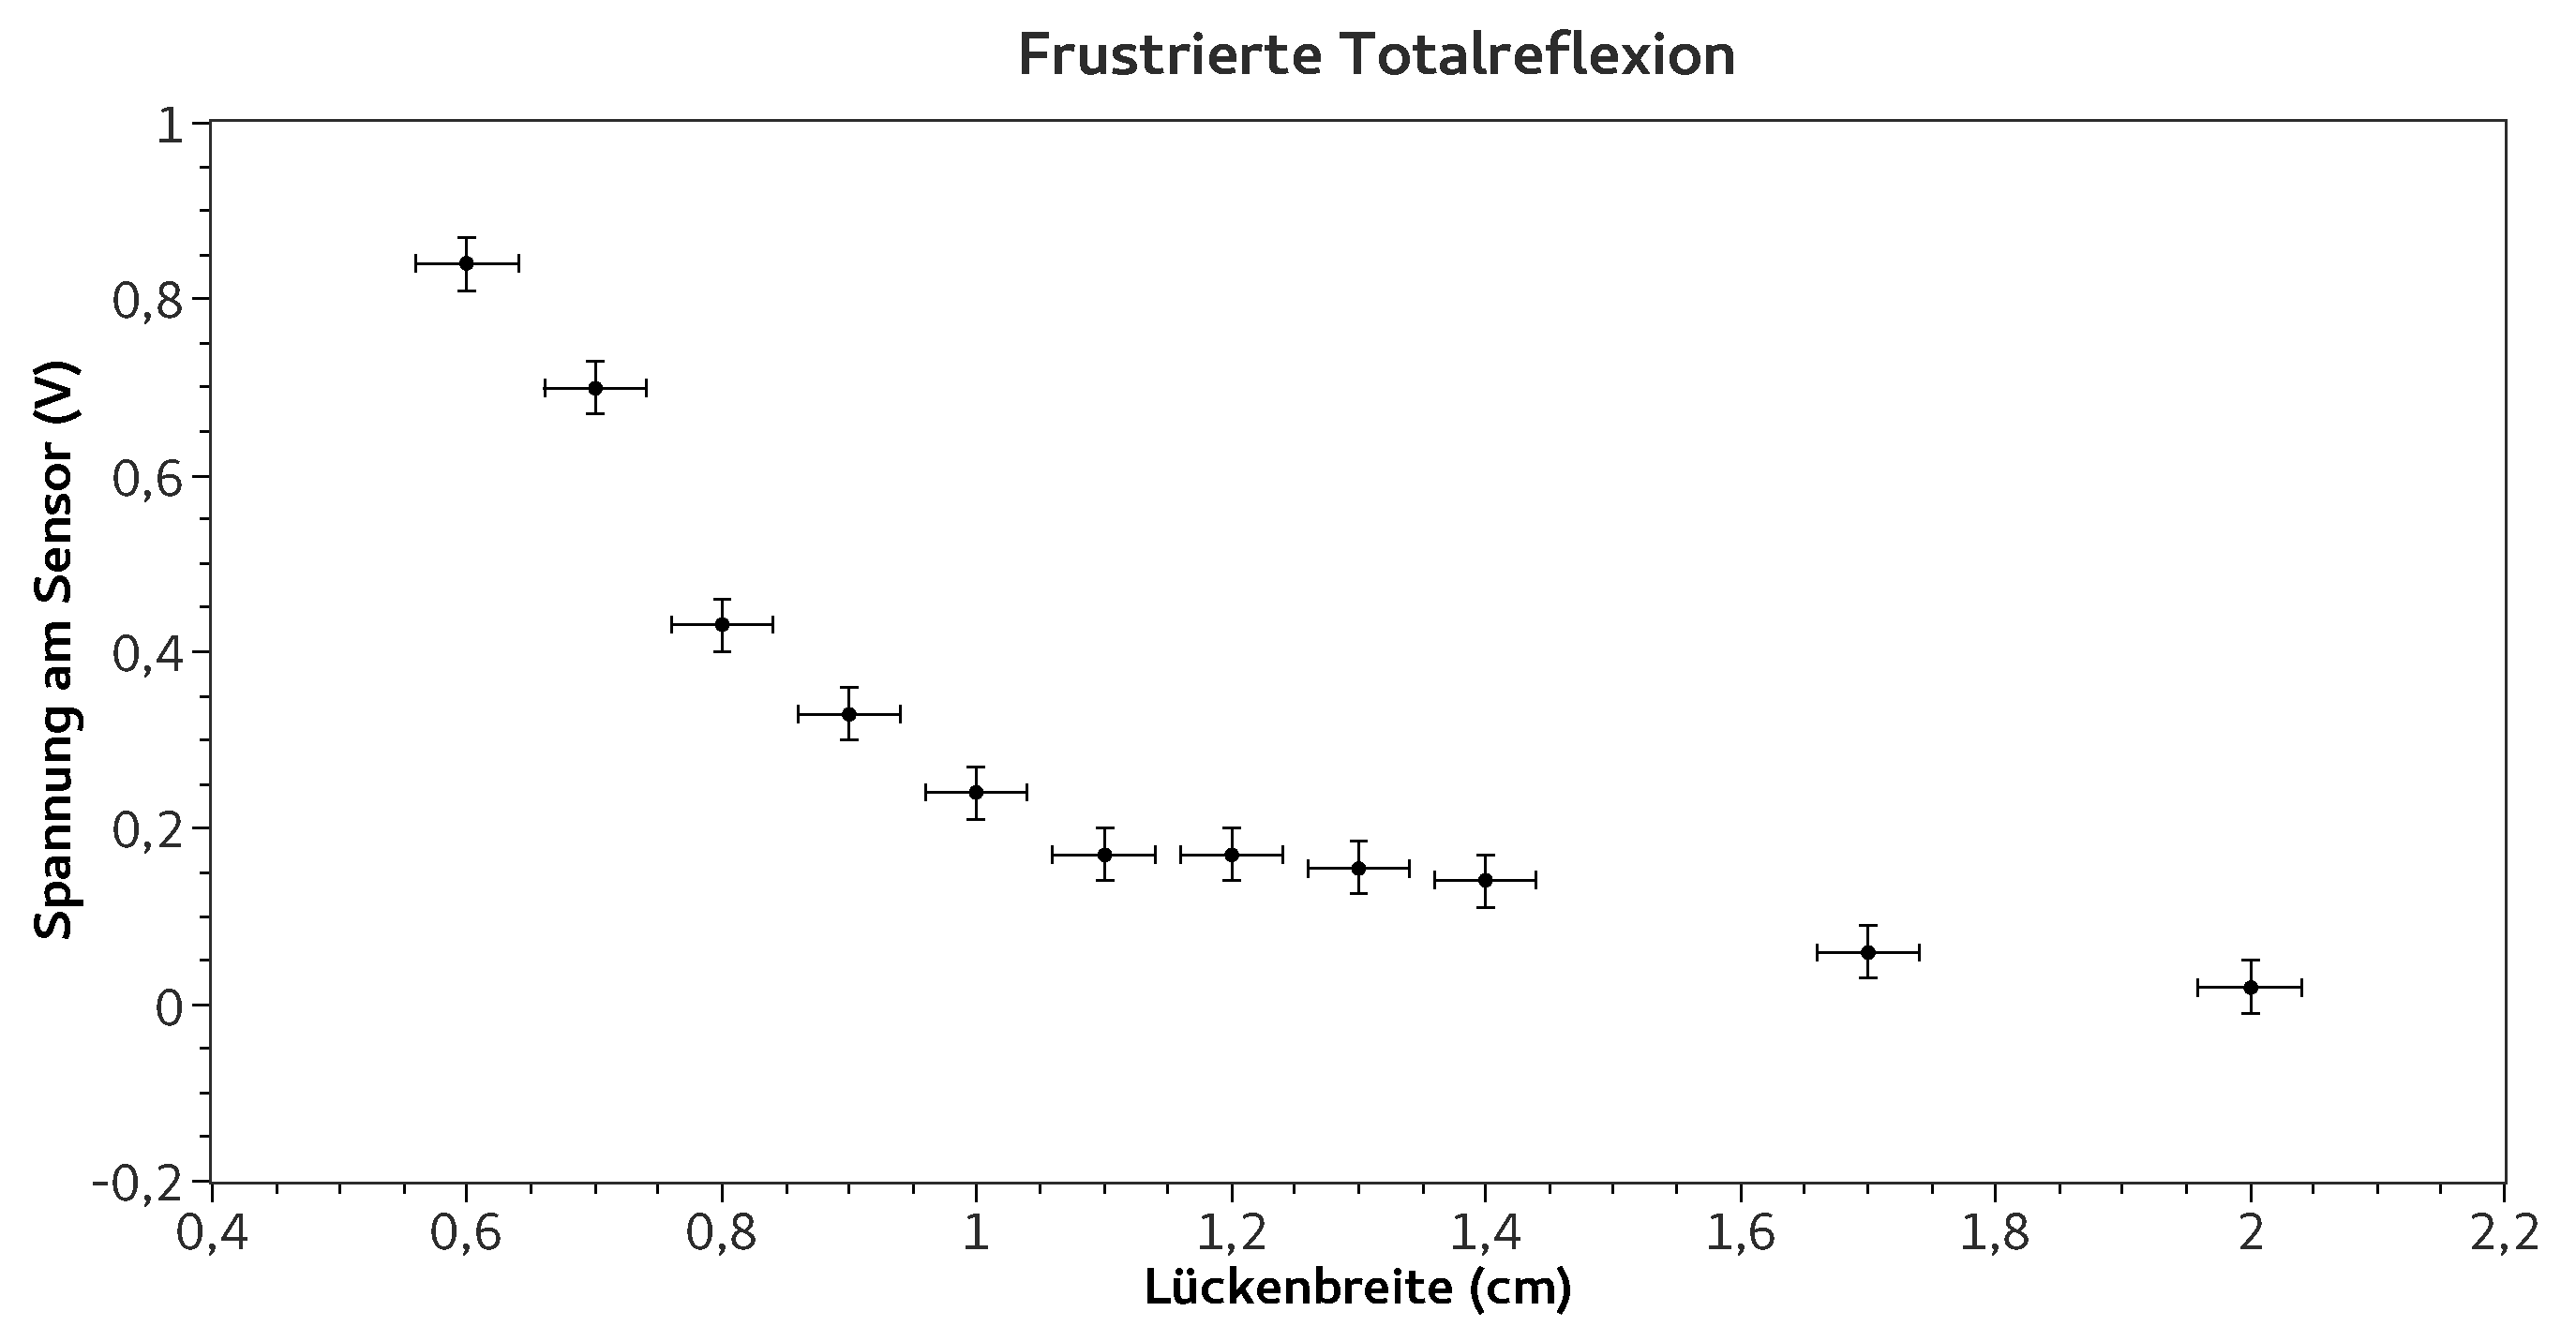
\includegraphics[width=0.7\textwidth]{fig_frust_total}
		\centering
		\caption{Gemessene Intensität der transmittierten Strahlung nach zwei Halbzylindern bei variiertem Lückenabstand unter Totalreflexion. Die rote Funktion ist eine exponentiell abnehmender Fit.}
		\label{fig_frust_total}
		\centering
	\end{figure}

	\subsubsection{Bragg-Reflexion}
	Die Braggsche Reflexionsbedingung lautet:
	\begin{equation}
		2d \sin(\alpha) = n \lambda
	\end{equation}
	Wobei n = 1,2,... ist.
	In \cref{fig_bragg} wird die Reflexion bei einem Winkel von \SI{55,+-1}{\degree} maximal.
	Folglich ist 
	\begin{equation*}
		\frac{\lambda}{2sin(\alpha)} = \SI{1,93+-0,06}{cm}.
	\end{equation*}
	Es kann nicht ausgeschlossen werden, dass für kleinere $\alpha$ ein weiteres Maximum existiert.
	Deshalb ist eine eindeutige Bestimmung der Gitterkonstante nicht möglich.
	Beim direkten Messen der Abstände der Kugeln im Schaumstoff ergab sich ein Abstand $d$ von \SI{3,875+-0,2}{cm}, woraus ersichtlich ist, dass das Maximum bei \SI{55}{\degree} dem bei $n=2$ entspricht, da $2\cdot\SI{1,93}{cm} \approx d$. 
	\begin{figure}[H]
		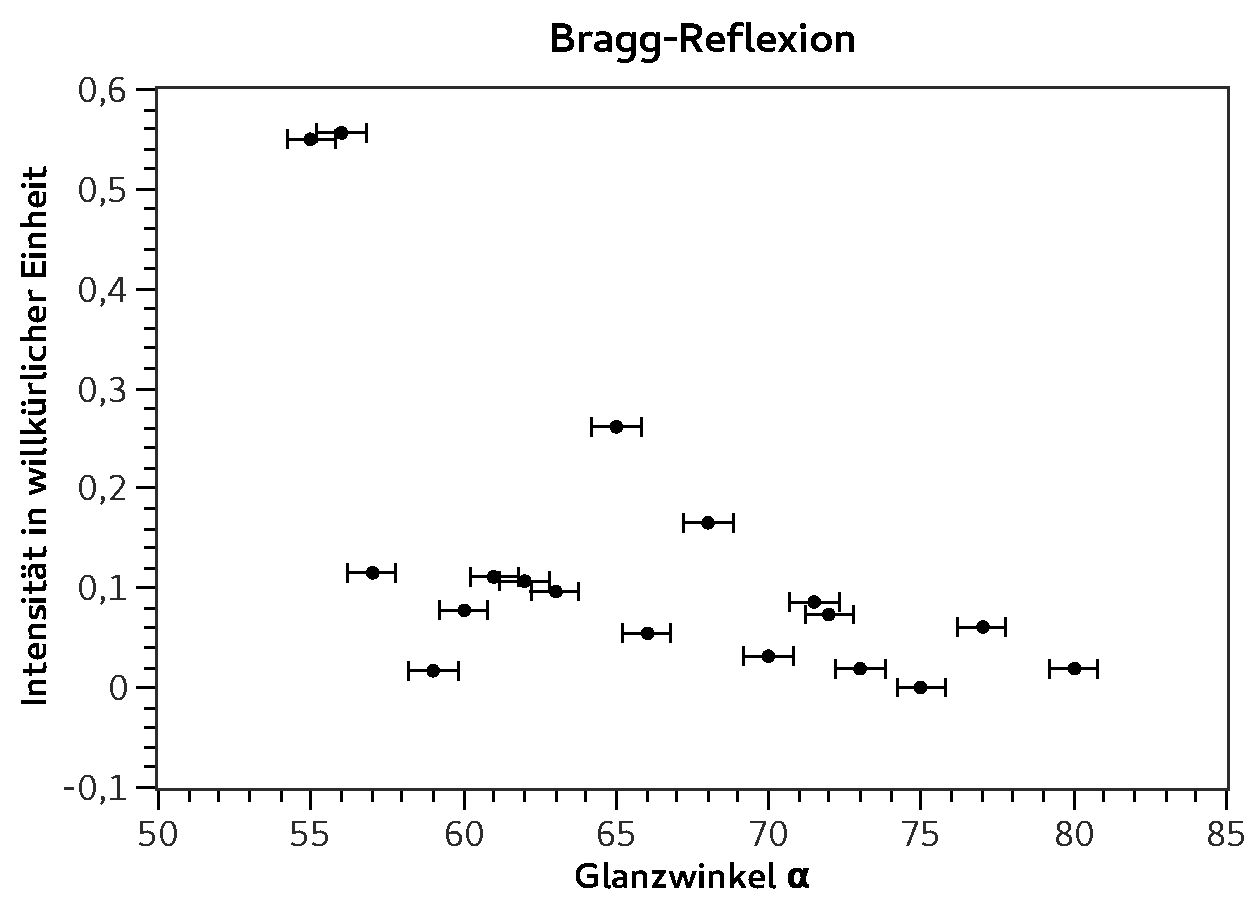
\includegraphics[width=0.7\textwidth]{fig_bragg}
		\centering
		\caption{Gemessene Intensität der Reflexionsstrahlung im Ausfallswinkel $2\alpha$ bei einem Einfallswinkel von $\alpha$.}
		\label{fig_bragg}
		\centering
	\end{figure}
	\subsection{Diskussion}
	%TODO Bezug/Nutzen oder sonst was
	%TODO auch hier die Hypothese wiederholen
	%TODO keine Messwerte hier, nach manchen Menschen, zumindest "direkt" erstellte Diagramme net hier, auch wenn Lesbarkeit-bla
	
	Wie in \crefrange{fig_74cm}{fig_114cm} zu erkennen ist, lassen sich die Strahlenprofile durch eine Gauß-Kurve beschreiben.
	Auf Grundlage dessen lässt sich bestätigen, dass der Strahl dem Konzept des Gauß-Strahls entspricht, dass Strahlen, die näherungsweise linear von der Quelle aus in der Breite wachsen, beschreibt. %TODO Ich hoffe mal das kommt von Wiki, ich weiß nämlich nix richtig/falsch. (Lasergaußstrahl wächst auch linear. dunno?)
	Die daraus folgende zur Strahlrichtung orthogonale Abweichung des Quellpunkts ist für die kleineren drei Entfernungen von Sender zu Empfänger (\cref{tab_xc}) kleiner als der Fehler, weshalb angenommen werden kann, dass in dieser Richtung keine messbare Verschiebung der Quelle gegenüber der Position des Senders vorliegt.
	Dies wäre auch aufgrund der Symmetrie des Aufbaus in dieser Richtung nicht zu erwarten gewesen.
	Die etwas größere Abweichung von ca. \SI{3}{mm} bei großem Abstand in X-Richtung lässt sich durch die wackelnde Halterungen von Sender und Empfänger erklären.
	Dass der Fokus vor dem Sender liegt, lässt sich durch die Geometrie des Senders erklären.
	Dieser hat sich zur Antenne verjüngende Metallwände, die die Strahlung reflektieren können.
	Durch die Interferenz dieser Wellen liegt der Fokus des Gauß-Strahls im Bereich der Öffnung der Mikrowellenquelle.
	
	Die Wellenlänge liegt mit \SI{3,14\pm 0,05}{cm} innerhalb des Bereiches des elektromagnetischen Spektrums, in dem man Wellen als Mikrowellen bezeichnet.
	
	Gemäß \cite{PVC-Brech} wird der Brechungsindex von PVC bei \SI{1,54}{} erwartet.
	Dies liegt innerhalb der Messfehler der Messwerte für Bestrahlung der runden Seite des Halbzylinders (\SI{1,56\pm 0,05}{}) und für Bestrahlung der flachen Seite (\SI{1,57 \pm 0,05}{}).
	Da diese Messwerte aus dem Einfallswinkel und Ausfallswinkel größter Intensität gemäß des Snelliusschen Brechungsgesetzes bestimmt wurden, lässt sich hier das Snelliussche Brechungsgesetz als nicht widerlegt ansehen. %TODO okay?
	
	In \cref{fig_bragg} lässt sich erkennen, dass die Intensität der durch beide Halbzylinder transmittierten Strahlung die bei frustrierter Totalreflexion erwartete exponentielle Abnahme mit der Breite der Lücke zwischen den beiden Hohlzylindern widerspiegelt.
	Insofern lässt sich sagen, dass hier das Phänomen der frustrierten Totalreflexion beobachtet werden konnte.
	
	Bei der Bragg-Reflexion konnte nicht das Maximum für $n=1$ gemessen werden, aber das für $n=2$.
	Da dieser Wert des Gitterabstandes aber mit dem durch direkte Messung mit einem Geodreieck innerhalb der Unsicherheiten übereinstimmt, kann die Vermutung, dass Bragg-Reflexion aufgetreten ist, bestätigt werden. 
	 
	
	
	\section{Schlussfolgerung}
	%TODO Rückgriff auf Hypothese und drittes Nennen dieser
	Die Hypothesen konnten vollständig bestätigt werden.
	Es konnte gezeigt werden, dass die Strahldivergenz der vorliegenden Mikrowellenquelle durch das Konzept des Gauß-Strahls beschrieben werden kann und daraus konnte die Position des Fokus relativ zum Sender bestimmt werden. %TODO Jatiza meinte halt auch Strahlenddivergenz ist niergends so richtig definiert, deswegen bin ich für Strahlenprofil anstatt Divergenz.
	Hierbei wurde festgestellt, dass der Fokus des Gaus-Strahls im Bereich des Ausgangs der Quelle liegt.
	Der gemessene Brechungsindex von PVC gemäß des Snelliusschen Brechungsgesetzes schloss den gemäß der Literatur erwarteten Wert in seinen Unsicherheiten ein, weshalb das Snelliussche Brechungsgesetz für Mikrowellen nicht widerlegt werden konnte.
	Außerdem ließ sich der exponentielle Abfall der Intensität mit dem Abstand zwischen zwei Hohlzylindern bei frustrierter Totalreflexion experimentell nachweisen, was die Annahme, dass hier frustrierte Totalreflexion zu beobachten war, bestätigen.
	Zuletzt ließ sich ein Maximum bei Bragg-Reflexion auflösen und zeigen, dass der daraus berechnete Gitterabstand im Schaumstoffblock mit dem direkt gemessenen übereinstimmt.
	Eine Auflösung von weiteren Maxima hätte einen Messarm (die Schiene mit dem Empfänger) mit weniger Spiel vorausgesetzt, da dies die Messung stark beeinträchtigt hat. %TODO meh, schärfer ja aber ich weiß net ob wir bei ca. 30° oder so net was hätten messen können. (Aber der Empfänger mittelt ja iwie immer übern großen bereih der Öffnung)
	
	\printbibliography
\end{document}
